\documentclass{a0poster}
\usepackage{fancytikzposter} % here most of the things are defined
% change parameters only after this line
\usepackage[margin=\margin cm, paperwidth=84.1cm, paperheight=118.9cm]{ geometry}
\usepackage{polski}
\usepackage{setspace}
\usepackage[T1]{fontenc}
\usepackage[utf8]{inputenc} 
\usetemplate{5}
\title{\Huge{PISA 2012 - How to succeed in Maths?}}
\author{Marcin Kosiński, Norbert Ryciak, Marta Sommer,  Faculty of Mathematics and Information Sciences on WUT}
\begin{document}
\AddToShipoutPicture{\BackgroundPicture}
\noindent
\begin{tikzpicture}
\initializesizeandshifts
\titleblock{60}{3}
\blocknode{ Here's our recipe! }{\Large{ Have you ever wondered how to be successful at Maths \\ and what you should change to improve your Maths results? \\
If you have, please consider our tips for success.}}%{\includegraphics[width=0.9\textwidth]{}}
\blocknode{1. Do emotions matter?}{ \Large{ \ \\ To start, here’s the obvious: those who like Maths tend to do better at it. But what makes us partial to the queen of
sciences?} \\ \ \\ 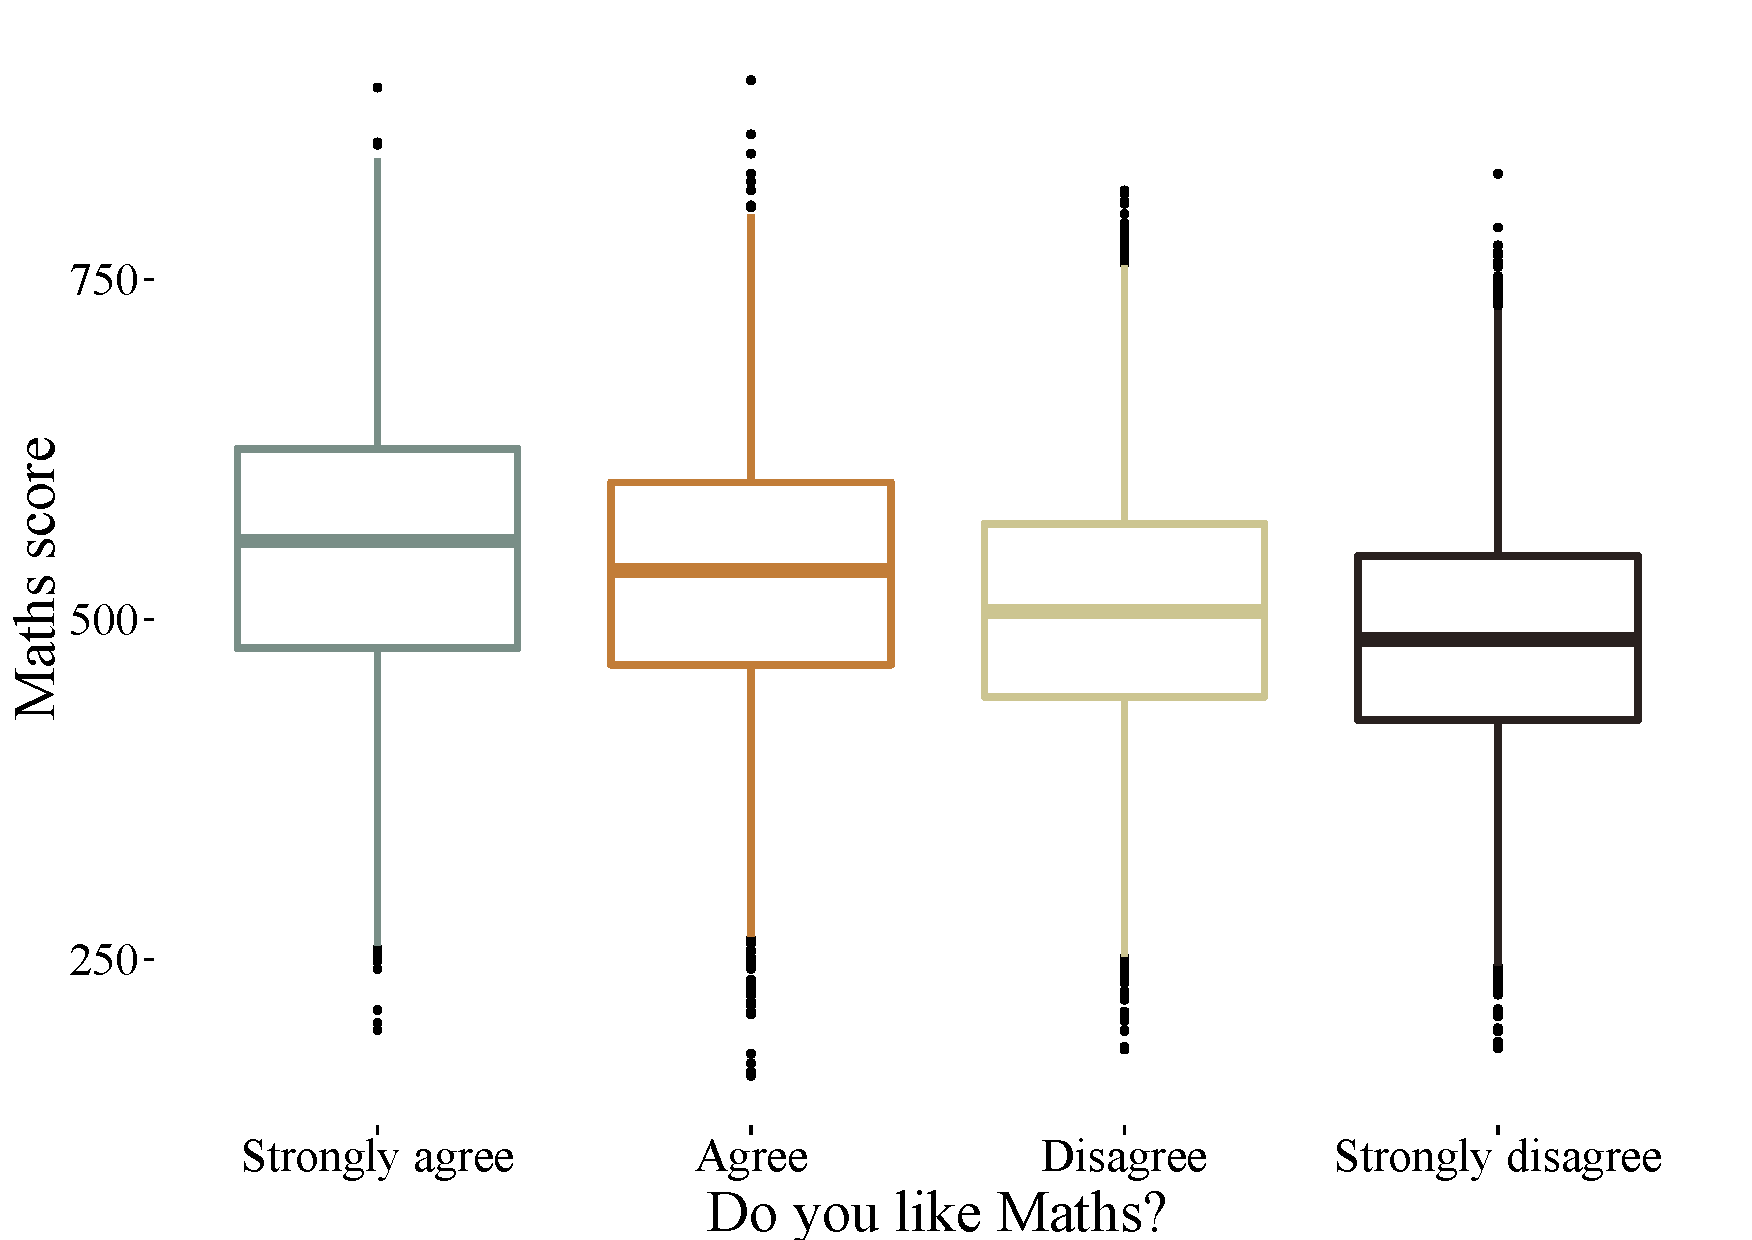
\includegraphics[width=0.99\textwidth]{graphs/wyk1lewy.pdf} \\ \ }
\blocknode{3. Is determination important?}{ \Large{ \ \\ … you should not give up. Determination does influence exam results! And what about consistent study?
} \\ \ \\ 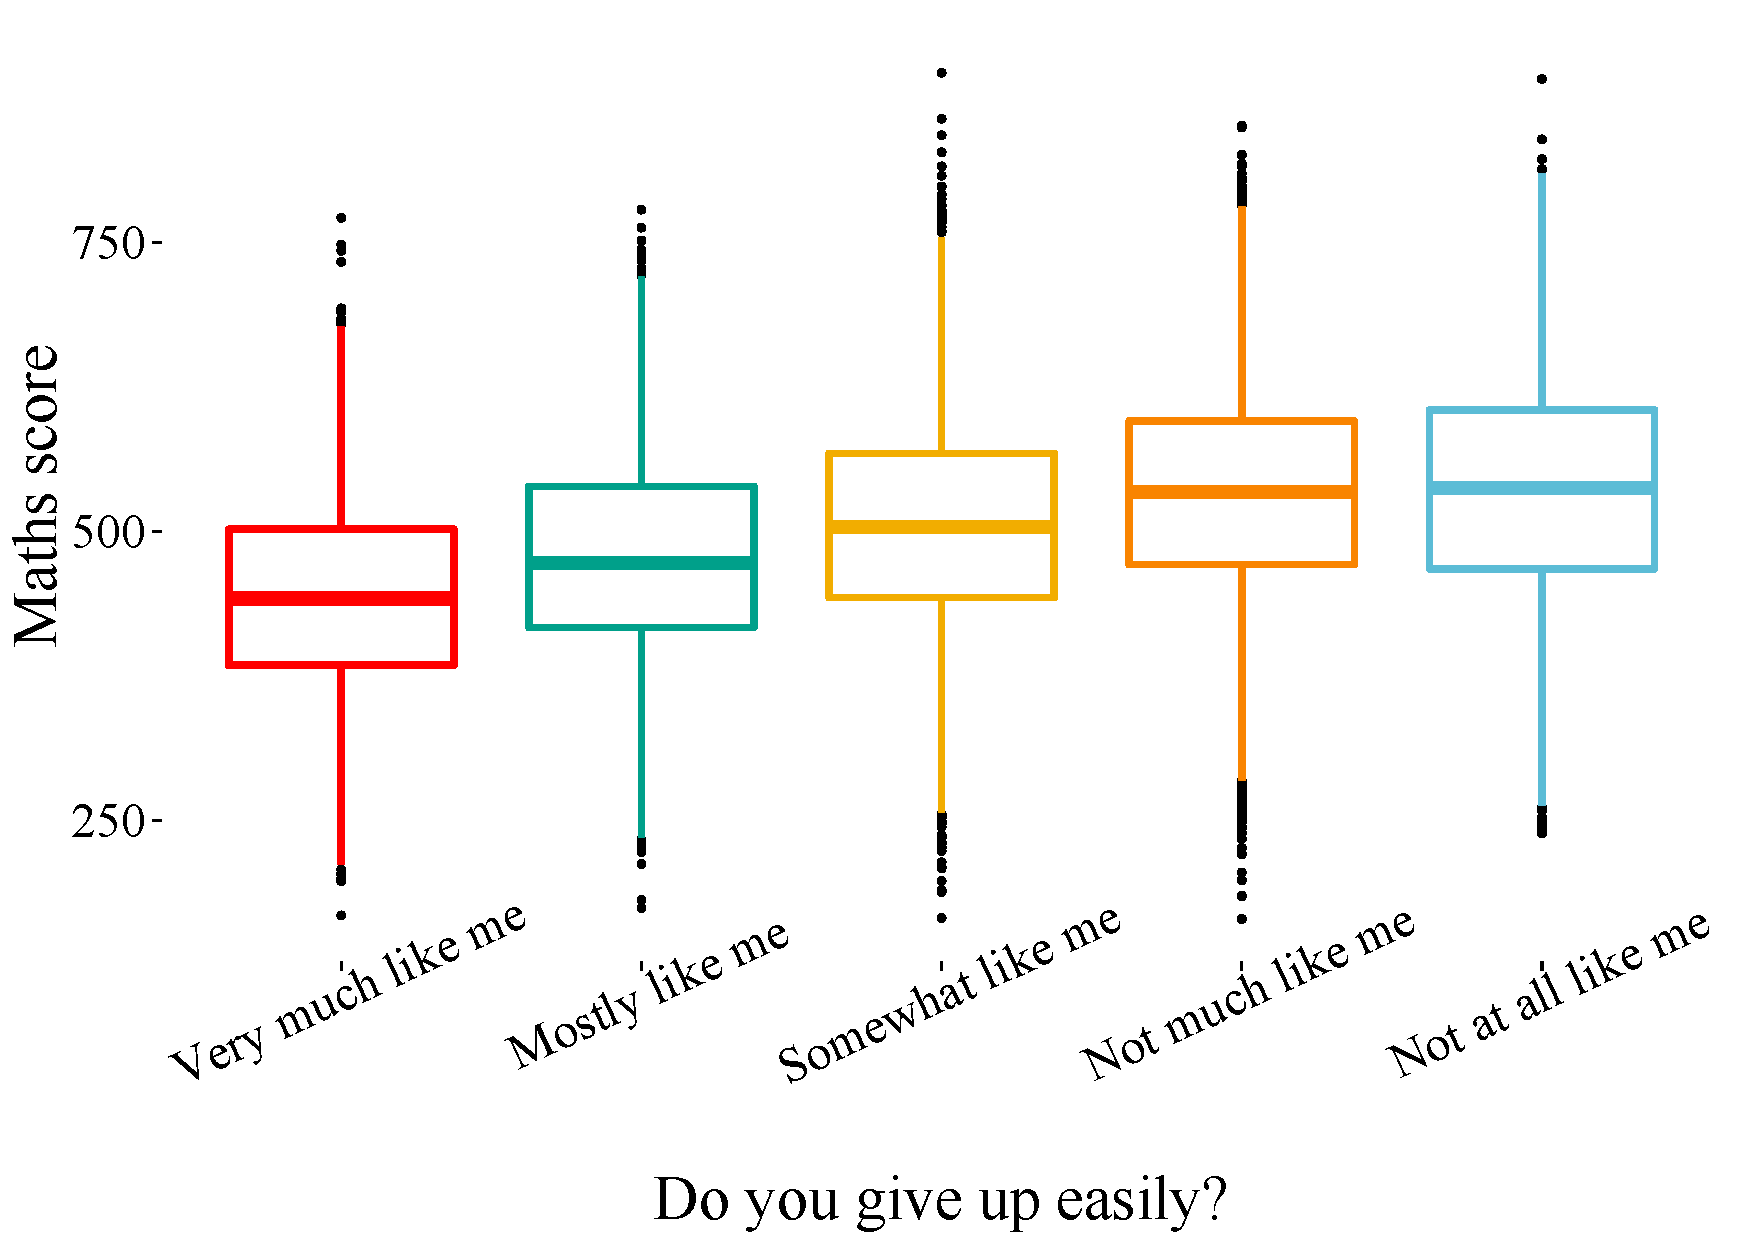
\includegraphics[width=0.99\textwidth]{graphs/wyk2lewy.pdf} }



\startsecondcolumn
\blocknode{Codes and Software}{ \centering \textbf{http://github.com/MarcinKosinski/PISAvis - codes} \\
\textbf{https://github.com/karthik/wesanderson - palletes } \\
\textbf{http://ggplot2.org/ - graphs } \\
\textbf{http://www.oecd.org/pisa/keyfindings/pisa-2012-results.htm - data set} }
\blocknode{2. How does parents' attitude affect their children?}{\Large{ \  \\ It turns out that whether you like Maths depends on whether your parents do. Aren’t your parents too keen on it?
Well, you’re off to a little worse start. However…} \\ \ \\ 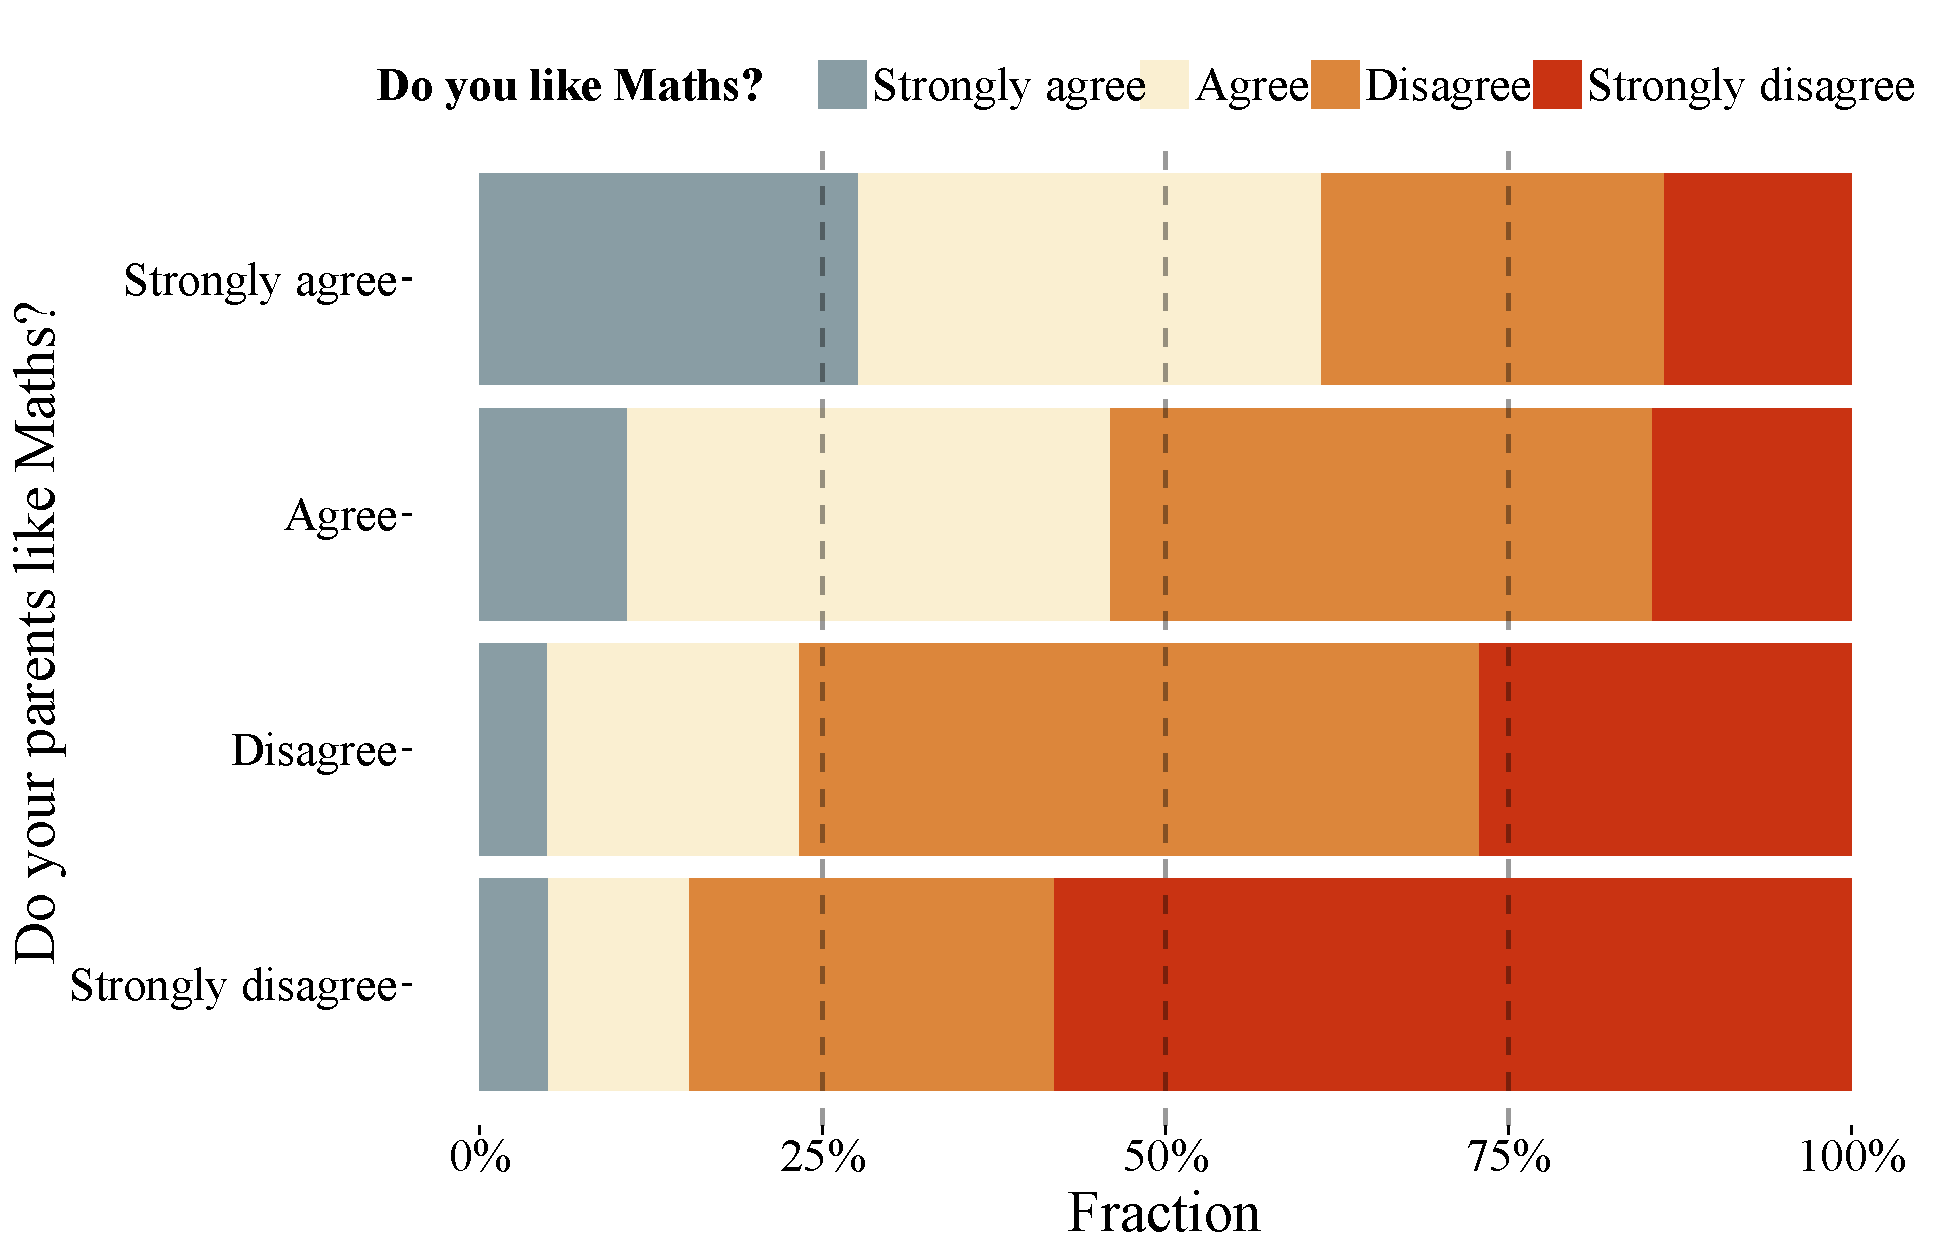
\includegraphics[width=0.99\textwidth]{graphs/wyk1prawy.pdf}}
\blocknode{4. Is it worth to pay attention in classes? }{
\Large{\ \\ 
The conclusion seems straightforward: if you do your homework and pay attention in class, you get good results.
However, just working at home, even if systematic, is not enough. If you don’t pay attention in class, you’re setting
yourself behind.}
 \\
 \begin{center}
 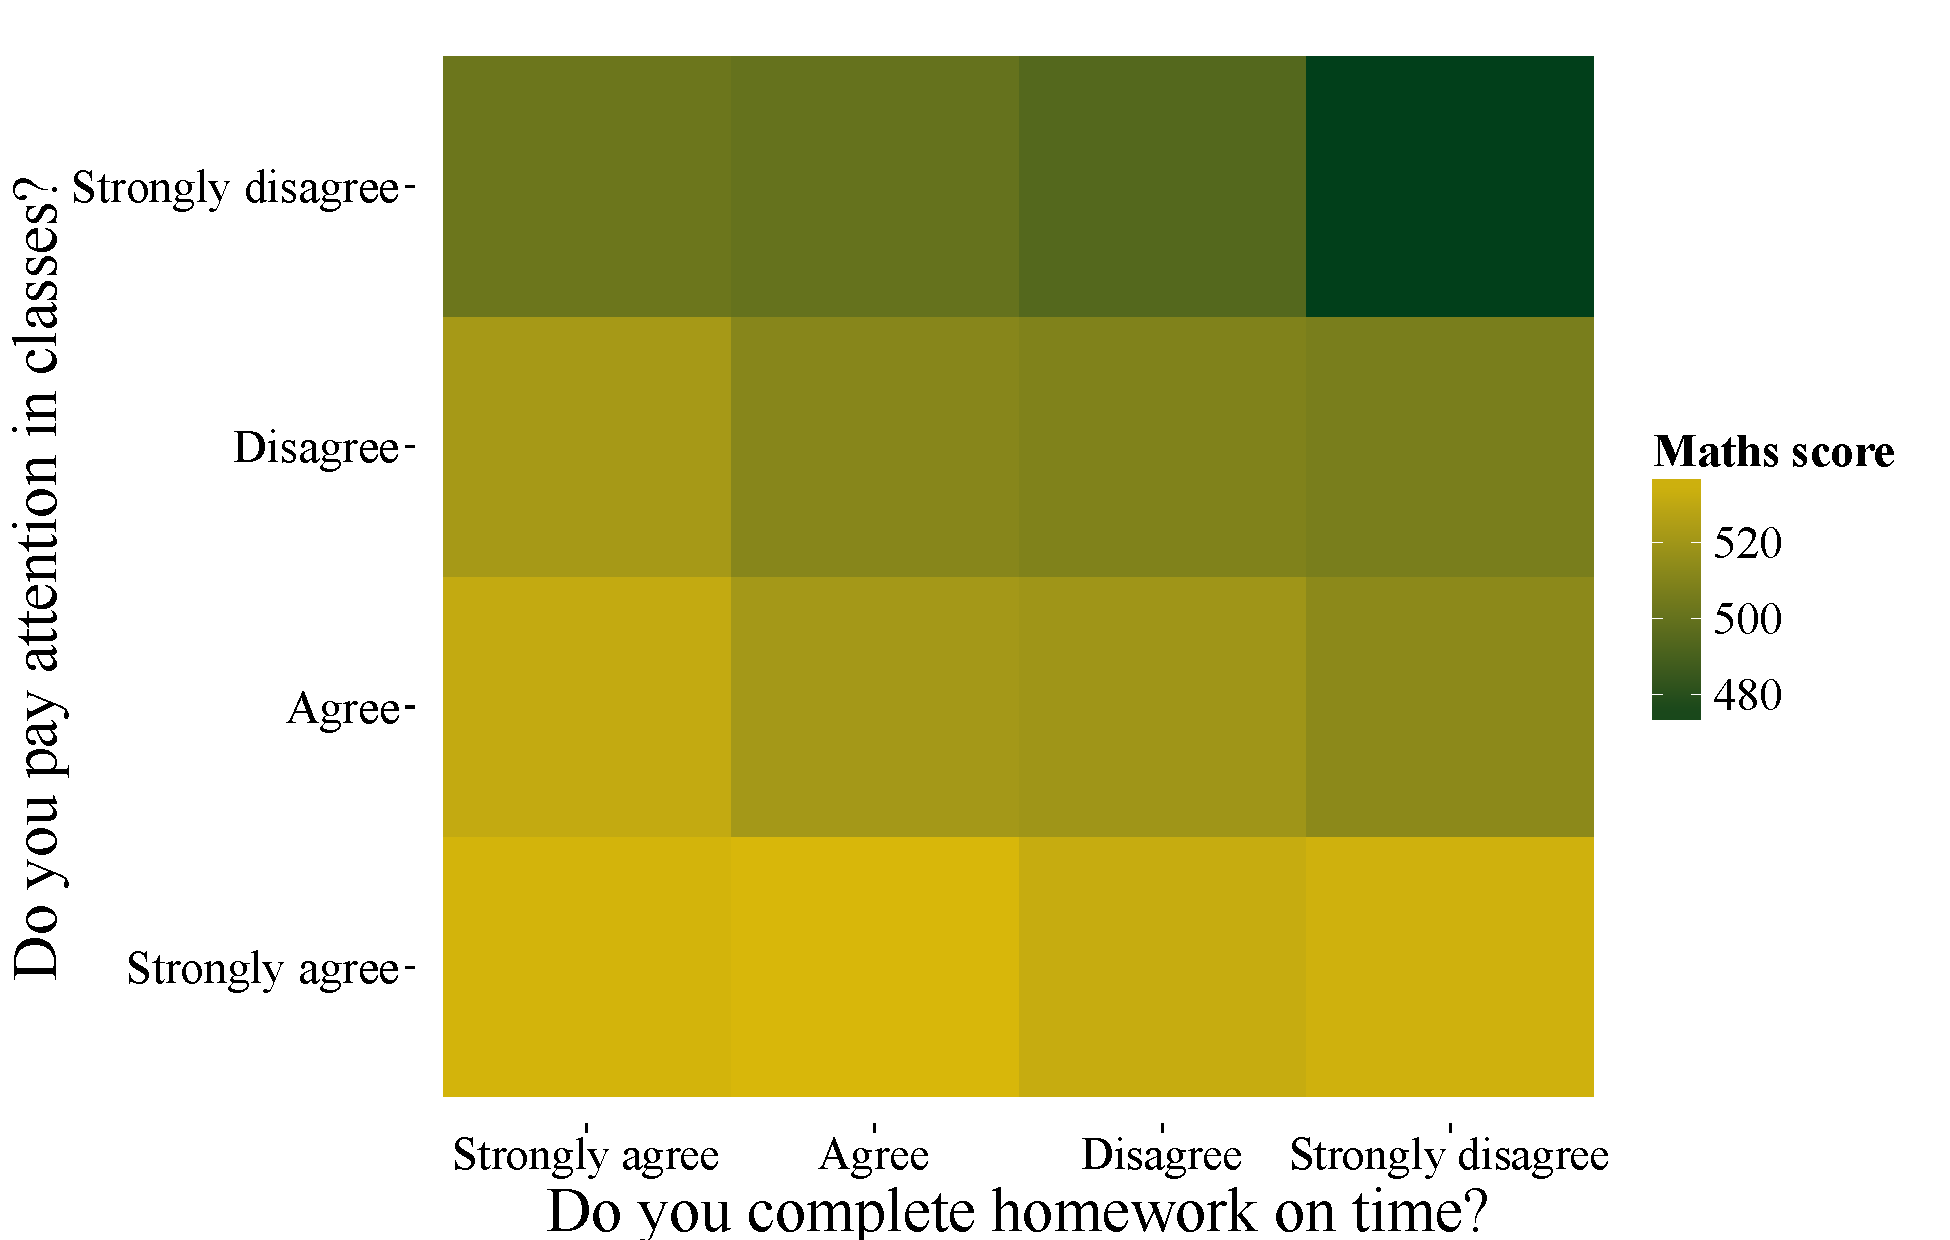
\includegraphics[width=0.99\textwidth, height=20cm]{graphs/wyk3prawy.pdf}
 \end{center}  }
 \plainblock[1]{($(currenty) +(-9,1)$)}{35}{Remember!} %
  {It pays if you grow to like Maths. Also, it’s worth your while to study, both at school and at home. And lastly, you
should never throw in the towel. Good luck!

  }


\end{tikzpicture}
\end{document}
